% v2-acmtog-sample.tex, dated March 7 2012
% This is a sample file for ACM Transactions on Graphics
%
% Compilation using 'acmtog.cls' - version 1.2 (March 2012), Aptara Inc.
% (c) 2010 Association for Computing Machinery (ACM)
%
% Questions/Suggestions/Feedback should be addressed to => "acmtexsupport@aptaracorp.com".
% Users can also go through the FAQs available on the journal's submission webpage.
%
% Steps to compile: latex, bibtex, latex latex
%
% For tracking purposes => this is v1.2 - March 2012
\documentclass{acmtog} % V1.2

%\acmVolume{VV}
%\acmNumber{N}
%\acmYear{YYYY}
%\acmMonth{Month}
%\acmArticleNum{XXX}
%\acmdoi{10.1145/XXXXXXX.YYYYYYY}

\acmVolume{28}
\acmNumber{4}
\acmYear{2009}
\acmMonth{September}
\acmArticleNum{106}
\acmdoi{10.1145/1559755.1559763}

\begin{document}

\title{Approximate Convolutional network for image classifier} % title

\author{XINYUAN LU {\upshape and} YUXUAN JIANG
\affil{Shanghai Jiao Tong University}}



\maketitle





\section{Introduction}

\looseness-1Nowadays, more and more convolutional network models are proposed to get more representative features, such as densenet and resnet. And the deeper network is, the more powerful it is. But there is an phenomenon that different image actually do not need same depth to get feature map. Take image classify for example. Image would be thought ��hard�� or ��easy�� , just like red wine in figure.1. And easy image can be classified correctly through shallow network, while hard ones need deep. It is wasteful to pass all images though whole deep net. So we consider an architecture not only saving resource(especially time), but also guarantee accuracy. It is similar to approximate computing, but there are some differences.

Comparing with traditional approximate computing, approximate classifier with more complex formulation. And each the feature map extracted in each layer can be use as the basic of next layer. We are inspired by $\cite{name1}$. They simple way is to admit image exit early. In some layers maybe the features is representative enough to have a correct prediction, we don't have to extract it again. So it is different with traditional approximate computing, here the approximate and precise computing are the different part of one model, instead of different models.

Actually the two architecture they proposed has obvious drawbacks, while the idea is excellent: create a gate function to judge when one image can be considered extracted enough, and then the result can be returned as final result.

Then we use new architecture MSDnet $\cite{name2}$. It is proposed not for approximate computing, but actually it is useful. It solve all the drawback of two architecture. And it has different classifiers in different layer, which is suitable for us to try the "early-exit" strategy.

Then we try the traditional gate function on MSDnet and mix the gate function and MSDnet in different ways. And we proposed one new formulation of gate function. Then we set up our new hybrid architecture. It performs well in the CIFAR-10. It guarantee the accuracy and speed up at almost 34%.

Furthermore, we utilize gate function on other architecture and find it also make contribution to ��mismatch��. It is an phenomenon some easy image can be classified by shallow net but can't by deep net. And we try our gate function to solve it.



\section{Background and Motivation}

%
\looseness-1As we describe in the introduction, we notice that resnet18 can get about 91 accuracy in CIFAR-10. Resnet-110 can get 93 while spend almost three times of time. That means, there are many images do not need deep network.

So we come up with an idea to find a way to judge whether one image need to go through deep network. Easy would pass through shallow net to save time, hard image pass deep net to guarantee accuracy. It is similar idea with traditional approximate computing.

And the difference is, we do not have a precise answer. However deep our network is, we can not guarantee it can predict all test set correctly. We only have a high-accuracy model designed regardless of consideration of resource.


\begin{figure}
  \centering
  % Requires \usepackage{graphicx}
  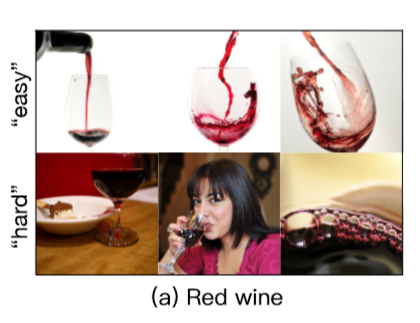
\includegraphics[scale=0.8]{1.png}
  \caption{hard and easy}
\end{figure}


\section{Relative work}
\subsubsection{Gate function}
We mentioned that $\cite{name1}$ and $\cite{name3}$ proposed two ways to try. But they all have drawbacks.

Left one: an adaptive network selection method, takes a set of pre-trained DNNs, each with a different cost and accuracy trade-off, and arranges them in a directed acyclic graph ,with the cheapest model first and the most expensive one last. After each model, our gate function would judge whether it can return or should jump to more complex model. Its drawback is Hard pictures may go though too much network and cost a lot of resource. And it is waste to extract features again and again


Right one is  an adaptive early-exit strategy that allows easy examples to bypass some of the network��s layers.But early layer are lack of coarse-level features.So it can't predict well. Also, in training, our cost function would be sum of all classifiers. And early classi?ers interfere with later classifiers. To make early layers to have a better prediction, early layer would be modified to have a better ability of compressing image, while information loses.

But they tried a novel way to judge it. They use a function to judge whether it would leave the architecture early. It is called gate function. It is the key of our approximate classifier.

\subsubsection{MSDnet}

So we turn to another architecture $MSDnet$,$\cite{name2}$. This architecture designed to get a good result at any limitation of resource. We find it useful to do approximate classifier. Figure 3 is its architecture. It use Multi-scale feature maps. The feature maps at a particular layer and scale are computed by concatenating the results of one or two convolutions: 1. the result of a regular convolution applied on the same-scale features from the previous layer (horizontal connections) and, if possible, 2. the result of a strided convolution applied on the finer-scale feature map from the previous layer (diagonal connections). So the early classifier would also perform well. What��s more, if an earlier layer collapses information to generate short-term features, the lost information can be recovered through the direct connection to its preceding layer by using Dense connectivity.






\begin{figure*}
  \centering
  % Requires \usepackage{graphicx}
  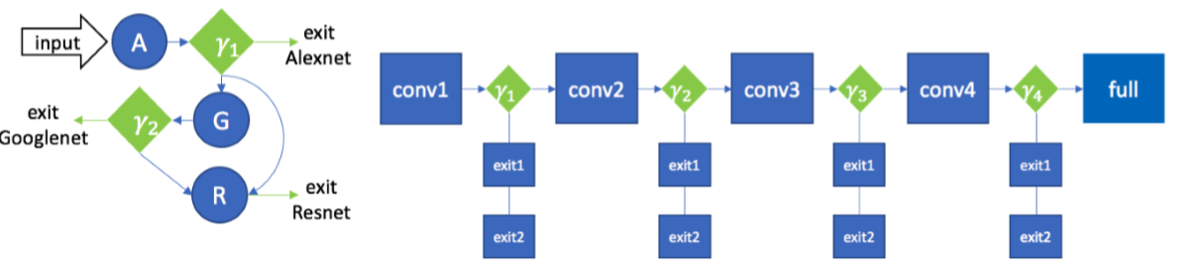
\includegraphics[scale=0.5]{2.png}
  \caption{two architecture}\label{two architecuture}
\end{figure*}



\begin{figure*}
  \centering
  % Requires \usepackage{graphicx}
  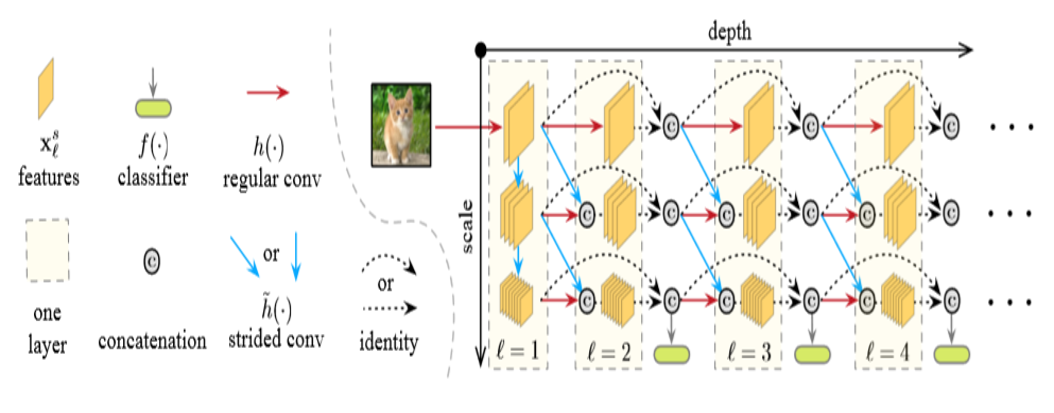
\includegraphics[scale=0.5]{3.png}
  \caption{MSDnet}\label{}
\end{figure*}

\section{Problem Formulation}
\label{sub:models_of_pupil_dynamics}
Given a input image x, we have some pre-trained models,$f_0,f_1,f_2...$, to utilize for a prediction.Where, the model, $f_0$,,is a high prediction-cost(HPC) model, which is either a priori known, or which we train to high-accuracy regardless of cost considerations. We would like to learn some alternative low prediction-cost (LPC) model $f_1,f_2,f_3$��. They have different cost and different accuracy. Notice in MSDnet, LPC are different part of HPC.

Then we propose a gate function $h(x)$, it would tell us how "hard" x is.So the total cost of x is:
\begin{equation}\label{1}
  C_{total}(x) = C_f(x) + C_h(x)
\end{equation}

We can't define the precise formulation of $C_f$ and $C_h$, it would change with change of formulation of $h(x)$. And the total cost of all the test set is:

\begin{equation}\label{2}
  C_{all}=\sum_{x}{C_{total}(x)}+\gamma * E
\end{equation}

Where $E$ is the error rate of all testset, and $\gamma$ is the hyperparameter to balance the tradeoff between accuracy and cost.

Our goal is to minimize $C_{all}$

\section{The Proposed Method}
\label{sec:proposed_model}


Actually, what we should do is to formulate a good function $h$. And we first pretrain a MSDnet in trainset. And then we tried two ways to attach gate function to origin MSDnet. Then for each input x, we would have $p_i(x),h_i(x)$ and $t_i(x)$, which means the max possibility of  prediction in layer i,time cost of $h(x)$ at layer i and all time of $f(x)$ passing through i layers.
\subsubsection{Inside the MSDnet}
If we want to deal with each feature map after each layer, it would be too complex and it is obvious the term $C_h(x)$ would be too large.
What's more, with more layer added to get an ability to classify difficult image, we have to add more gate function if we attach gate inside the MSDnet. To minimize the $C_h(x)$, there is a limitation of complexity of gate function. So, add it after each Classifier would a good strategy.  Then its architecture would be like figure 4.
\begin{figure}
  \centering
  % Requires \usepackage{graphicx}
  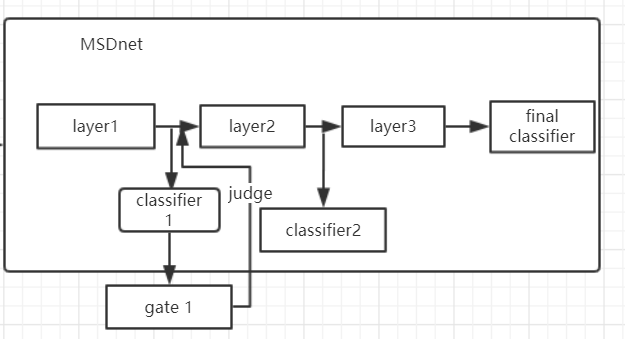
\includegraphics[scale=0.5]{4.png}
  \caption{gate inside the MSDnet}\label{}
\end{figure}

So $C_h(x)$ and $C_f(x)$ of equation 1 would become :
\begin{eqnarray*}\label{3}
    D=\mathop{\arg\min}_{d:p_d(x)>\alpha} \ \ \| \mathrm{d} \|.\\
    C_h(x)=\sum_{i=1}^Dh_i(x)\\
    C_f(x)=t_D(x)
\end{eqnarray*}

where D means the depth we judge for image x to leave our architecture. $\alpha$ is a hypeparameter we set.

\subsubsection{Before the MSDnet}
Now we turn to another idea. We do the experiment (would shown in EXPERIMENT), finding it performs badly if we attach gate inside. And we find it hard for this architecture to predict "hard" image. For example, if we use it to predict "hard" image in figure, the one describing woman drinking red wine. The possibility of class red wine and class woman would be close. They are up and down in about 0.48. Maybe in some layers possibility women would greater than $\alpha$, and if it is earlier than class red wine does, we get a wrong answer. In face, almost wrong answer caused by this reason.

In the final analysis, our gate function is too weak to judge whether image is hard or easy. But as we discussed before, it would cost too much resource to use complex function if we attach it inside. So we try another architecture: we use a more powerful but cost more function, train it and put it before MSDnet. We just use it once in the prediction. It would tell the MSDnet when it should let image to leave.

It is hard to create such function because it is a hard problem to judge image easy or hard even in human's sensibility. We have many data but no idea about function, so we turn to neural network. Convolutional neural network use convolutional kernel to extract local features, and score them in the last full-connective layer. We want to use the Redundancy of network. If we label some easy images using one label, we guess network would use easy kernel (such as identity mapping), and full-connect would score all features. So easy ones would become one class. Hard ones would become another class. And we divide some level from easy to hard and label all images. Now it becomes another image classify problem.

But how to label it? In fact, we can't distinguish it is hard for human to judge or hard for our MSDnet to judge. Since we use MSDnet to predict, we use it to label its level. Using the thought of Bayesian formulation, we would assume we know the final result when we label it. That means, we would know the final prediction answers $C_whole$ using whole network and its possibility $P_whole$. Once in some layers D, its possibility of class $C_whole$ is greater than one absolute number $\alpha$ and relative number $\beta * P_whole$ ,then we label it in depth D, that means:
\begin{eqnarray*}\label{3}
    D=\mathop{\arg\min}_{d:PS_d(C_whole)>\alpha \quad and\quad PS_d(C_whole)>\beta * P_whole} \ \ \| \mathrm{d} \|.\\
\end{eqnarray*}

where $PS_d(C)$ means the possibility of class C in layer d.

And $C_h(x)$ and $C_f(x)$ would be:
\begin{eqnarray*}\label{3}
    C_h(x)=T\\
    C_f(x)=t_D(x)
\end{eqnarray*}

the time of h(x) would be a constant T. And figure 5 is our last architecture.
\begin{figure*}
  \centering
  % Requires \usepackage{graphicx}
  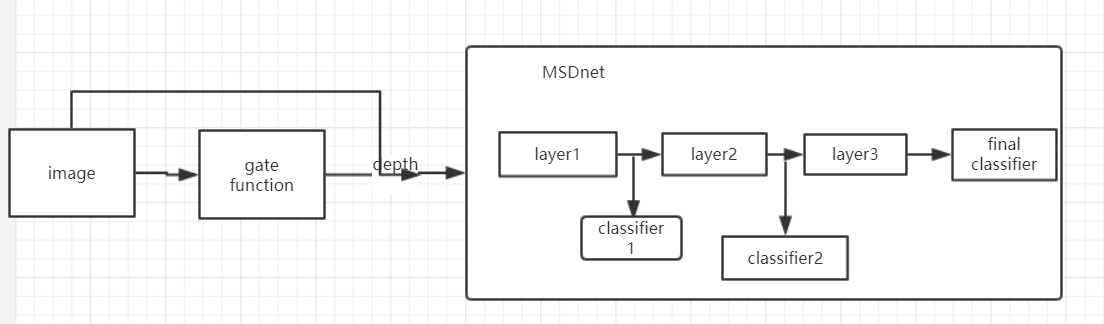
\includegraphics[scale=0.5]{5.png}
  \caption{hybrid architecture}\label{two architecuture}
\end{figure*}

\subsubsection{Mismatch}
I notice there is an phenomenon that after trained, some picture can be classified by shallow network but can't classified by deep network, which I call it "mismatch". I explain it that to adapt the whole data set, especially some hard images, the deep network has to modify its kernel, which cause it unable to classify some easy images. Now we have a gate function, if we use it to judge whether one image is hard or easy, and pass easy ones to shallow net, and pass hard ones to deep net. Then our architecture would not only save time, but also improve total accuracy!

\section{Experiment}
\subsubsection{Architecture In CIFAR-10}
We do our two architectures in CIFAR-10. In first architecture, we set $\alpha$ 0.5. This number means this class is the most possible one. Then predict in the test set.

Then the second architecture. We set $\alpha$ 0.5 and $\beta$ 0.99 to label image. We chose resnet18 for gate function because it is powerful enough but would not cost too much time. We notice that in this way to label, almost images are labeled 0, which means almost images are thought easy and can be classified correctly using only small number of layers. To have a good training result, I abandon some level 0 images. And put rest images (about 30000) to resnet18 to train.

After training our resnet, we test our hybrid architecture in the test set.

Table I is our final result.\\

\begin{table}
\centering
\caption{result.}
\begin{tabular}{cccc}
\hline
Type&Top1&Top5&Time\\
\hline
Classifier0&90.800&99.740&95.06\\
\hline
Classifier1&92.330&99.800&125.38\\
\hline
Classifier2&93.180&99.750&154.83\\
\hline
Classifier3&93.760&99.750&183.68\\
\hline
Classifier4&94.140&99.780&203.30\\
\hline
Classifier5&94.130&99.750&227.68\\
\hline
Classifier6&94.270&99.800&256.16\\
\hline
Classifier7&94.220&99.810&268.93\\
\hline
Classifier8&94.210&99.720&275.21\\
\hline
Classifier9&94.170&99.790&283.53\\
\hline
Hybrid&94.090&99.770&151.23\\
\hline
Anytime&91.110&99.720&120.37\\
\hline
\end{tabular}
\label{table:result}
\end{table}
The classifier number represents its depth. We pass all data until fixed depth to compare. Anytime is the first architecture. We can see it performs badly. Hybrid is the second architecture, it performs well. Its accuracy is almost equal to classifier 4, but speed up almost 34%

\subsubsection{Mismatch in CIFAR-10}
I use two pre-trained models, shallow one is resnet20, deep one is resnet110. First I test it on how many images they classify differently. Resnet20 has 234 images in advantage(I call these images "shallow"), while resnet110 has 429 images(I call these images "deep").

Then I use gate to and get a simple architecture as figure 6.
\begin{figure}
  \centering
  % Requires \usepackage{graphicx}
  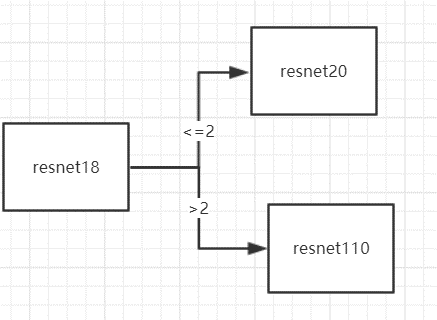
\includegraphics[scale=0.5]{6.png}
  \caption{simple hybrid}\label{two architecuture}
\end{figure}

The result is table II. I find gate label most "shallow" images small numbers, and label only some "deep" images big number. So it doesn't get ideal result. I think the reason is our gate function are trained for MSDnet rather than this special hybrid architecture. And maybe there is a difference between the "hard" images and "deep" images. I would do the work in the future.
\begin{table}
\centering
\caption{result2.}
\begin{tabular}{ccc}
\hline
Type&Top1&Time\\
\hline
Resnet110&93.680&160.41\\
\hline
Resnet20&91.730&37.58\\
\hline
Hybrid&92.100&47.377\\
\hline

\end{tabular}
\label{table:result}
\end{table}
\section{Conclusion}
To solve approximate classifier problem, we tried two hybrid architecture based on MSDnet to do approximate computing. Inside the architecture would limit its complexity, which would also limit its performance.The one putting gate function in front of MSDnet and using a complex gate function has a great improvement.It speeds up and guarantee the accuracy at the same time.

But in fact, we can't have a good explanation why gate function could work. It needs more job to validate whether it is caused by Redundancy of network. Also, maybe we could try more powerful gate function, such as Densenet. In fact, in the hybrid architecture,if the pre-classifier(here is resnet18) and main-part(MSDnet) have the same architecture, it would have an improvement. And gate function on mismatch doesn't give a ideal result. But actually CIFAR-10 is a simple data set, many images would be label at 0, which cause difficulty to train our gate function. I would do my experiment on more difficult data set such as IMAGENET. Also, I would do my work on mismatch.







% Bibliography
\bibliographystyle{ACM-Reference-Format-Journals}
\bibliography{acmtog-sample-bibfile}
                                % Sample .bib file with references that match those in
                                % the 'Specifications Document (V1.5)' as well containing
                                % 'legacy' bibs and bibs with 'alternate codings'.
                                % Gerry Murray - March 2012

\received{September 2008}{March 2009}



\end{document}
% End of v2-acmtog-sample.tex (March 2012) - Gerry Murray, ACM
